

\tikzset{every picture/.style={line width=0.75pt}} %set default line width to 0.75pt

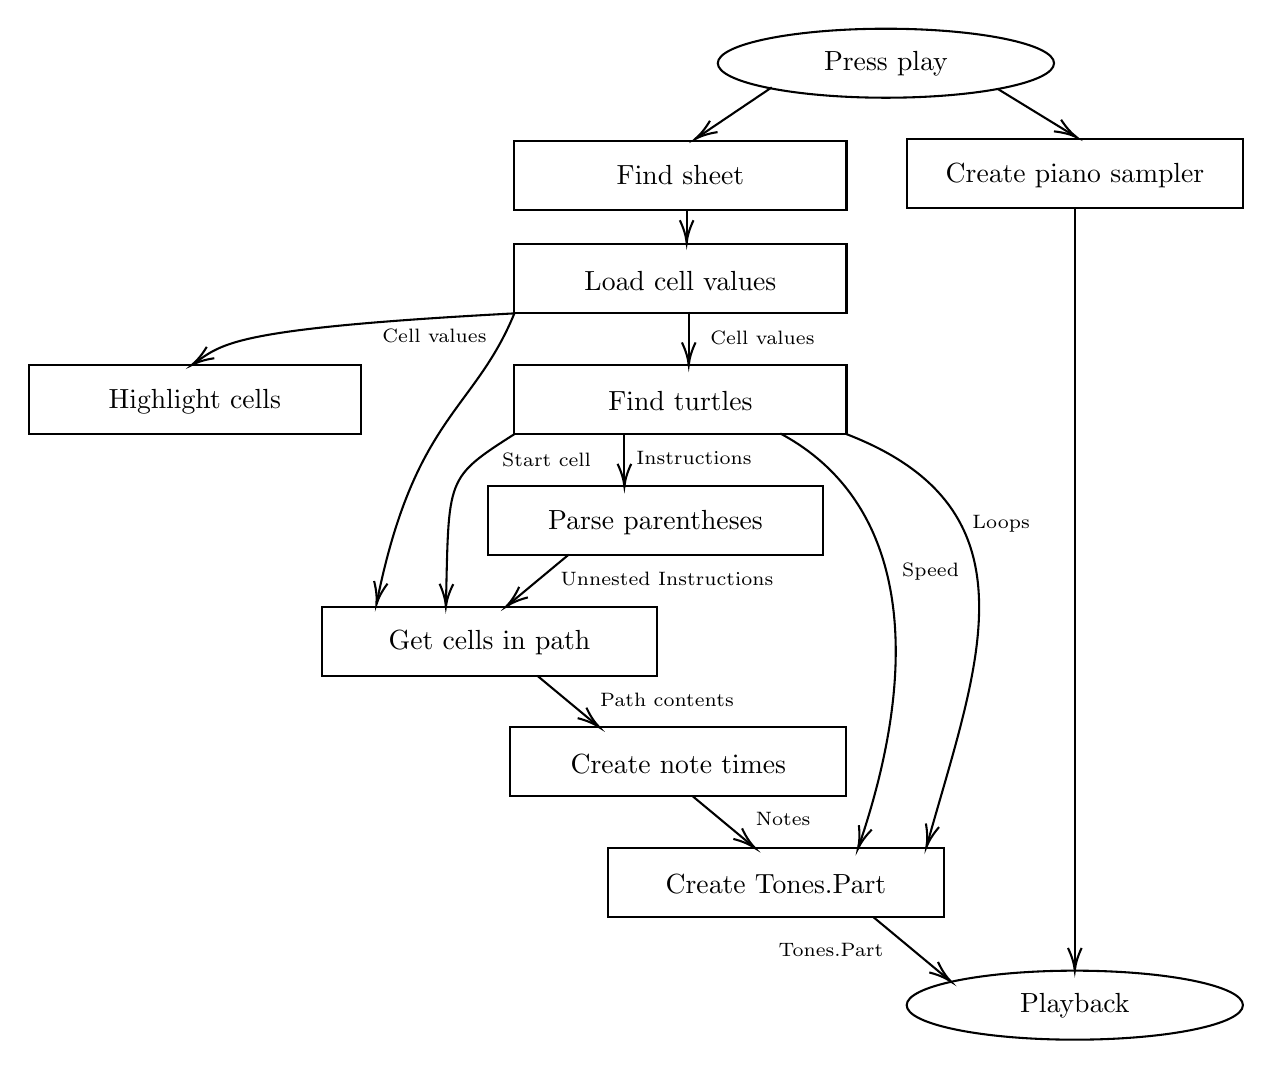
\begin{tikzpicture}[x=0.75pt,y=0.75pt,yscale=-1,xscale=1]
%uncomment if require: \path (0,604); %set diagram left start at 0, and has height of 604

%Shape: Rectangle [id:dp3390223975782729]
\draw   (244.5,60.03) -- (404.5,60.03) -- (404.5,93.28) -- (244.5,93.28) -- cycle ;

%Shape: Rectangle [id:dp7168559924493858]
\draw   (244.5,109.9) -- (404.5,109.9) -- (404.5,143.15) -- (244.5,143.15) -- cycle ;

%Shape: Rectangle [id:dp8835932361497658]
\draw   (433.7,59.2) -- (595.5,59.2) -- (595.5,92.44) -- (433.7,92.44) -- cycle ;

%Shape: Rectangle [id:dp9464422191216635]
\draw   (244.5,168.08) -- (404.5,168.08) -- (404.5,201.33) -- (244.5,201.33) -- cycle ;

%Shape: Rectangle [id:dp6384624480751633]
\draw   (231.6,226.27) -- (393.4,226.27) -- (393.4,259.51) -- (231.6,259.51) -- cycle ;

%Shape: Rectangle [id:dp2927464084046889]
\draw   (151.6,284.45) -- (313.4,284.45) -- (313.4,317.7) -- (151.6,317.7) -- cycle ;

%Shape: Rectangle [id:dp9052659554068596]
\draw   (242.6,342.63) -- (404.4,342.63) -- (404.4,375.88) -- (242.6,375.88) -- cycle ;

%Shape: Rectangle [id:dp5637329489183025]
\draw   (289.6,400.82) -- (451.4,400.82) -- (451.4,434.06) -- (289.6,434.06) -- cycle ;

%Curve Lines [id:da3917180624639185]
\draw    (244.5,201.33) .. controls (211.33,222.56) and (212.96,221.96) .. (211.54,282.59) ;
\draw [shift={(211.5,284.45)}, rotate = 271.37] [color={rgb, 255:red, 0; green, 0; blue, 0 }  ][line width=0.75]    (10.93,-3.29) .. controls (6.95,-1.4) and (3.31,-0.3) .. (0,0) .. controls (3.31,0.3) and (6.95,1.4) .. (10.93,3.29)   ;

%Straight Lines [id:da6961662223442007]
\draw    (297.5,201.33) -- (297.5,224.6) ;
\draw [shift={(297.5,226.6)}, rotate = 270] [color={rgb, 255:red, 0; green, 0; blue, 0 }  ][line width=0.75]    (10.93,-3.29) .. controls (6.95,-1.4) and (3.31,-0.3) .. (0,0) .. controls (3.31,0.3) and (6.95,1.4) .. (10.93,3.29)   ;

%Curve Lines [id:da9168950950169605]
\draw    (372.6,201) .. controls (431.31,232.42) and (442.88,304.83) .. (410.49,399.72) ;
\draw [shift={(410,401.15)}, rotate = 289.05] [color={rgb, 255:red, 0; green, 0; blue, 0 }  ][line width=0.75]    (10.93,-3.29) .. controls (6.95,-1.4) and (3.31,-0.3) .. (0,0) .. controls (3.31,0.3) and (6.95,1.4) .. (10.93,3.29)   ;

%Curve Lines [id:da7972588626438504]
\draw    (404.5,201.33) .. controls (499.03,237.72) and (467.32,313.11) .. (443.36,399.02) ;
\draw [shift={(443,400.32)}, rotate = 285.52] [color={rgb, 255:red, 0; green, 0; blue, 0 }  ][line width=0.75]    (10.93,-3.29) .. controls (6.95,-1.4) and (3.31,-0.3) .. (0,0) .. controls (3.31,0.3) and (6.95,1.4) .. (10.93,3.29)   ;

%Straight Lines [id:da6822022155717844]
\draw    (270.7,259.35) -- (242.04,283.17) ;
\draw [shift={(240.5,284.45)}, rotate = 320.27] [color={rgb, 255:red, 0; green, 0; blue, 0 }  ][line width=0.75]    (10.93,-3.29) .. controls (6.95,-1.4) and (3.31,-0.3) .. (0,0) .. controls (3.31,0.3) and (6.95,1.4) .. (10.93,3.29)   ;

%Straight Lines [id:da4884596231580207]
\draw    (255.5,317.7) -- (283.96,341.35) ;
\draw [shift={(285.5,342.63)}, rotate = 219.73] [color={rgb, 255:red, 0; green, 0; blue, 0 }  ][line width=0.75]    (10.93,-3.29) .. controls (6.95,-1.4) and (3.31,-0.3) .. (0,0) .. controls (3.31,0.3) and (6.95,1.4) .. (10.93,3.29)   ;

%Straight Lines [id:da9233366942734922]
\draw    (330.5,375.88) -- (358.96,399.54) ;
\draw [shift={(360.5,400.82)}, rotate = 219.73] [color={rgb, 255:red, 0; green, 0; blue, 0 }  ][line width=0.75]    (10.93,-3.29) .. controls (6.95,-1.4) and (3.31,-0.3) .. (0,0) .. controls (3.31,0.3) and (6.95,1.4) .. (10.93,3.29)   ;

%Straight Lines [id:da3670498457872964]
\draw    (417.5,434.06) -- (453.36,463.87) ;
\draw [shift={(454.9,465.15)}, rotate = 219.73] [color={rgb, 255:red, 0; green, 0; blue, 0 }  ][line width=0.75]    (10.93,-3.29) .. controls (6.95,-1.4) and (3.31,-0.3) .. (0,0) .. controls (3.31,0.3) and (6.95,1.4) .. (10.93,3.29)   ;

%Straight Lines [id:da28794703530347365]
\draw    (327.5,93.28) -- (327.5,107.23) ;
\draw [shift={(327.5,109.23)}, rotate = 270] [color={rgb, 255:red, 0; green, 0; blue, 0 }  ][line width=0.75]    (10.93,-3.29) .. controls (6.95,-1.4) and (3.31,-0.3) .. (0,0) .. controls (3.31,0.3) and (6.95,1.4) .. (10.93,3.29)   ;

%Straight Lines [id:da33376731250782754]
\draw    (328.5,142.32) -- (328.5,166.08) ;
\draw [shift={(328.5,168.08)}, rotate = 270] [color={rgb, 255:red, 0; green, 0; blue, 0 }  ][line width=0.75]    (10.93,-3.29) .. controls (6.95,-1.4) and (3.31,-0.3) .. (0,0) .. controls (3.31,0.3) and (6.95,1.4) .. (10.93,3.29)   ;

%Curve Lines [id:da2676626927985757]
\draw    (244.5,143.15) .. controls (225.1,190.29) and (196.29,192.83) .. (178.27,282.1) ;
\draw [shift={(178,283.45)}, rotate = 281.24] [color={rgb, 255:red, 0; green, 0; blue, 0 }  ][line width=0.75]    (10.93,-3.29) .. controls (6.95,-1.4) and (3.31,-0.3) .. (0,0) .. controls (3.31,0.3) and (6.95,1.4) .. (10.93,3.29)   ;

%Straight Lines [id:da024649031996502035]
\draw    (514.5,92.11) -- (514.5,457.83) ;
\draw [shift={(514.5,459.83)}, rotate = 270] [color={rgb, 255:red, 0; green, 0; blue, 0 }  ][line width=0.75]    (10.93,-3.29) .. controls (6.95,-1.4) and (3.31,-0.3) .. (0,0) .. controls (3.31,0.3) and (6.95,1.4) .. (10.93,3.29)   ;

%Shape: Ellipse [id:dp13505581605963868]
\draw   (433.5,476.45) .. controls (433.5,467.27) and (469.76,459.83) .. (514.5,459.83) .. controls (559.24,459.83) and (595.5,467.27) .. (595.5,476.45) .. controls (595.5,485.64) and (559.24,493.08) .. (514.5,493.08) .. controls (469.76,493.08) and (433.5,485.64) .. (433.5,476.45) -- cycle ;

%Shape: Ellipse [id:dp006287630832967794]
\draw   (342.5,22.62) .. controls (342.5,13.44) and (378.76,6) .. (423.5,6) .. controls (468.24,6) and (504.5,13.44) .. (504.5,22.62) .. controls (504.5,31.8) and (468.24,39.25) .. (423.5,39.25) .. controls (378.76,39.25) and (342.5,31.8) .. (342.5,22.62) -- cycle ;

%Straight Lines [id:da09048722077694915]
\draw    (368.5,34.26) -- (333.16,58.08) ;
\draw [shift={(331.5,59.2)}, rotate = 326.02] [color={rgb, 255:red, 0; green, 0; blue, 0 }  ][line width=0.75]    (10.93,-3.29) .. controls (6.95,-1.4) and (3.31,-0.3) .. (0,0) .. controls (3.31,0.3) and (6.95,1.4) .. (10.93,3.29)   ;

%Straight Lines [id:da9578993167654264]
\draw    (477.5,35.09) -- (513.79,57.32) ;
\draw [shift={(515.5,58.37)}, rotate = 211.49] [color={rgb, 255:red, 0; green, 0; blue, 0 }  ][line width=0.75]    (10.93,-3.29) .. controls (6.95,-1.4) and (3.31,-0.3) .. (0,0) .. controls (3.31,0.3) and (6.95,1.4) .. (10.93,3.29)   ;

%Shape: Rectangle [id:dp25073410390478523]
\draw   (10.5,168.08) -- (170.5,168.08) -- (170.5,201.33) -- (10.5,201.33) -- cycle ;

%Curve Lines [id:da2454539812308738]
\draw    (244.5,143.15) .. controls (108.92,150.37) and (104.17,157.58) .. (90.53,167.04) ;
\draw [shift={(89,168.08)}, rotate = 326.38] [color={rgb, 255:red, 0; green, 0; blue, 0 }  ][line width=0.75]    (10.93,-3.29) .. controls (6.95,-1.4) and (3.31,-0.3) .. (0,0) .. controls (3.31,0.3) and (6.95,1.4) .. (10.93,3.29)   ;


% Text Node
\draw (324.5,76.65) node  [align=left] {Find sheet};
% Text Node
\draw (324.5,127.35) node  [align=left] {Load cell values};
% Text Node
\draw (514.6,76.65) node  [align=left] {Create piano sampler};
% Text Node
\draw (324.5,185.54) node  [align=left] {Find turtles};
% Text Node
\draw (312.5,243.72) node  [align=left] {Parse parentheses};
% Text Node
\draw (232.5,301.9) node  [align=left] {Get cells in path};
% Text Node
\draw (323.5,360.09) node  [align=left] {Create note times};
% Text Node
\draw (370.5,418.27) node  [align=left] {Create Tones.Part};
% Text Node
\draw (514.5,476.45) node [] [align=left] {\textcolor[rgb]{0,0,0}{Playback}};
% Text Node
\draw (260,213.8) node  [align=left] {{\scriptsize Start cell}};
% Text Node
\draw (331,212.97) node  [align=left] {{\scriptsize Instructions}};
% Text Node
\draw (445,267.83) node  [align=left] {{\scriptsize Speed}};
% Text Node
\draw (479,244.55) node  [align=left] {{\scriptsize Loops}};
% Text Node
\draw (318,271.15) node  [align=left] {{\scriptsize Unnested Instructions}};
% Text Node
\draw (318,329.33) node  [align=left] {{\scriptsize Path contents}};
% Text Node
\draw (374,386.69) node  [align=left] {{\scriptsize Notes}};
% Text Node
\draw (397,449.86) node  [align=left] {{\scriptsize Tones.Part}};
% Text Node
\draw (206,153.95) node  [align=left] {{\scriptsize Cell values}};
% Text Node
\draw (423.5,22.62) node [] [align=left] {Press play};
% Text Node
\draw (364,154.78) node  [align=left] {{\scriptsize Cell values}};
% Text Node
\draw (90.5,185.54) node  [align=left] {Highlight cells};


\end{tikzpicture}
